\chapter{Metodi}
\label{cap:metodi}

\section{I dataset}
\label{sec:dataset}

Prima di poter valutare l'accuratezza dei modelli di machine learning proposti è necessario addestrarli con un apposito dataset; in questa tesi i modelli sono stati valutati utilizzandone due: uno creato ad hoc per questa tesi ed il Daily Living Activities (DLA) disponibile pubblicamente\cite{leotta2021daily}.

Al momento della ricerca non sono disponibili dataset pubblici contenenti dati di lavaggi e sanificazioni delle mani mediante segnali di accelerometro e giroscopio; per questo motivo si è deciso di crearne uno personalizzato raccogliendo i dati da una Inertial Measurement Unit (IMU) posizionata sul polso della mano dominante di quattro partecipanti durante attività di vita reale.

Per raccogliere i dati abbiamo utilizzato una IMU Shimmer3 equipaggiata con un accelerometro e un giroscopio tri-assale\cite{shimmer}; questo dispositivo, visibile in Figura \ref{fig:shimmer}, è progettato appositamente per essere indossato ed è spesso utilizzato nel monitoraggio delle attività nell'ambito delle scienze sportive e mediche. Al suo interno monta una serie di sensori wide-range con campionamento a 14 bit, range da $\pm2.0g$ fino a $\pm16.0g$ ed una sensitività da $1mg/LSB$ fino a $12mg/LSB$; lo Shimmer3 può essere considerato una buona rappresentazione delle IMU correntemente equipaggiate all'interno degli smartwatch commerciali. Il dispositivo indossabile è stato programmato per campionare il suo accelerometro e giroscopio ad una frequenza di 100Hz e salvare i dati raccolti in una SD-card interna. Per rimuovere il bias dei sensori il dispositivo è stato calibrato all'inizio della ricerca lasciandolo su una superficie piana per circa 30 secondi in modo da ottenere una traccia di calibrazione.
In Figura \ref{fig:acc-gyro-plot} vediamo un'esempio delle sei tracce di accelerometro e giroscopio raccolte durante un'attività di sanificazione delle mani.

\begin{figure}[!htb]
    \centering
    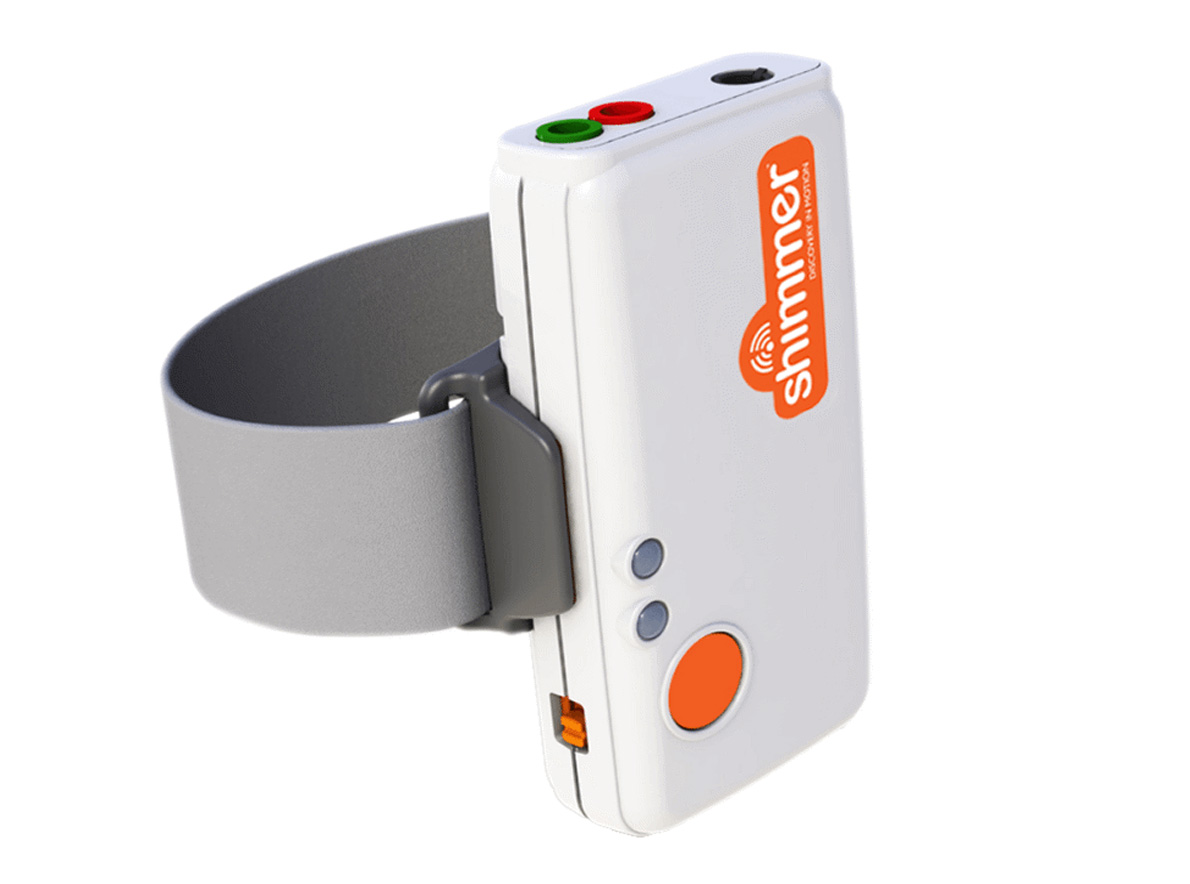
\includegraphics[width=.4\textwidth]{figure/shimmer.jpg}
    \caption{IMU Shimmer3 dotata di bracciale per essere indossata al polso dell'utente.}
    \label{fig:shimmer}
\end{figure}

\begin{figure}[!htb]
    \centering
    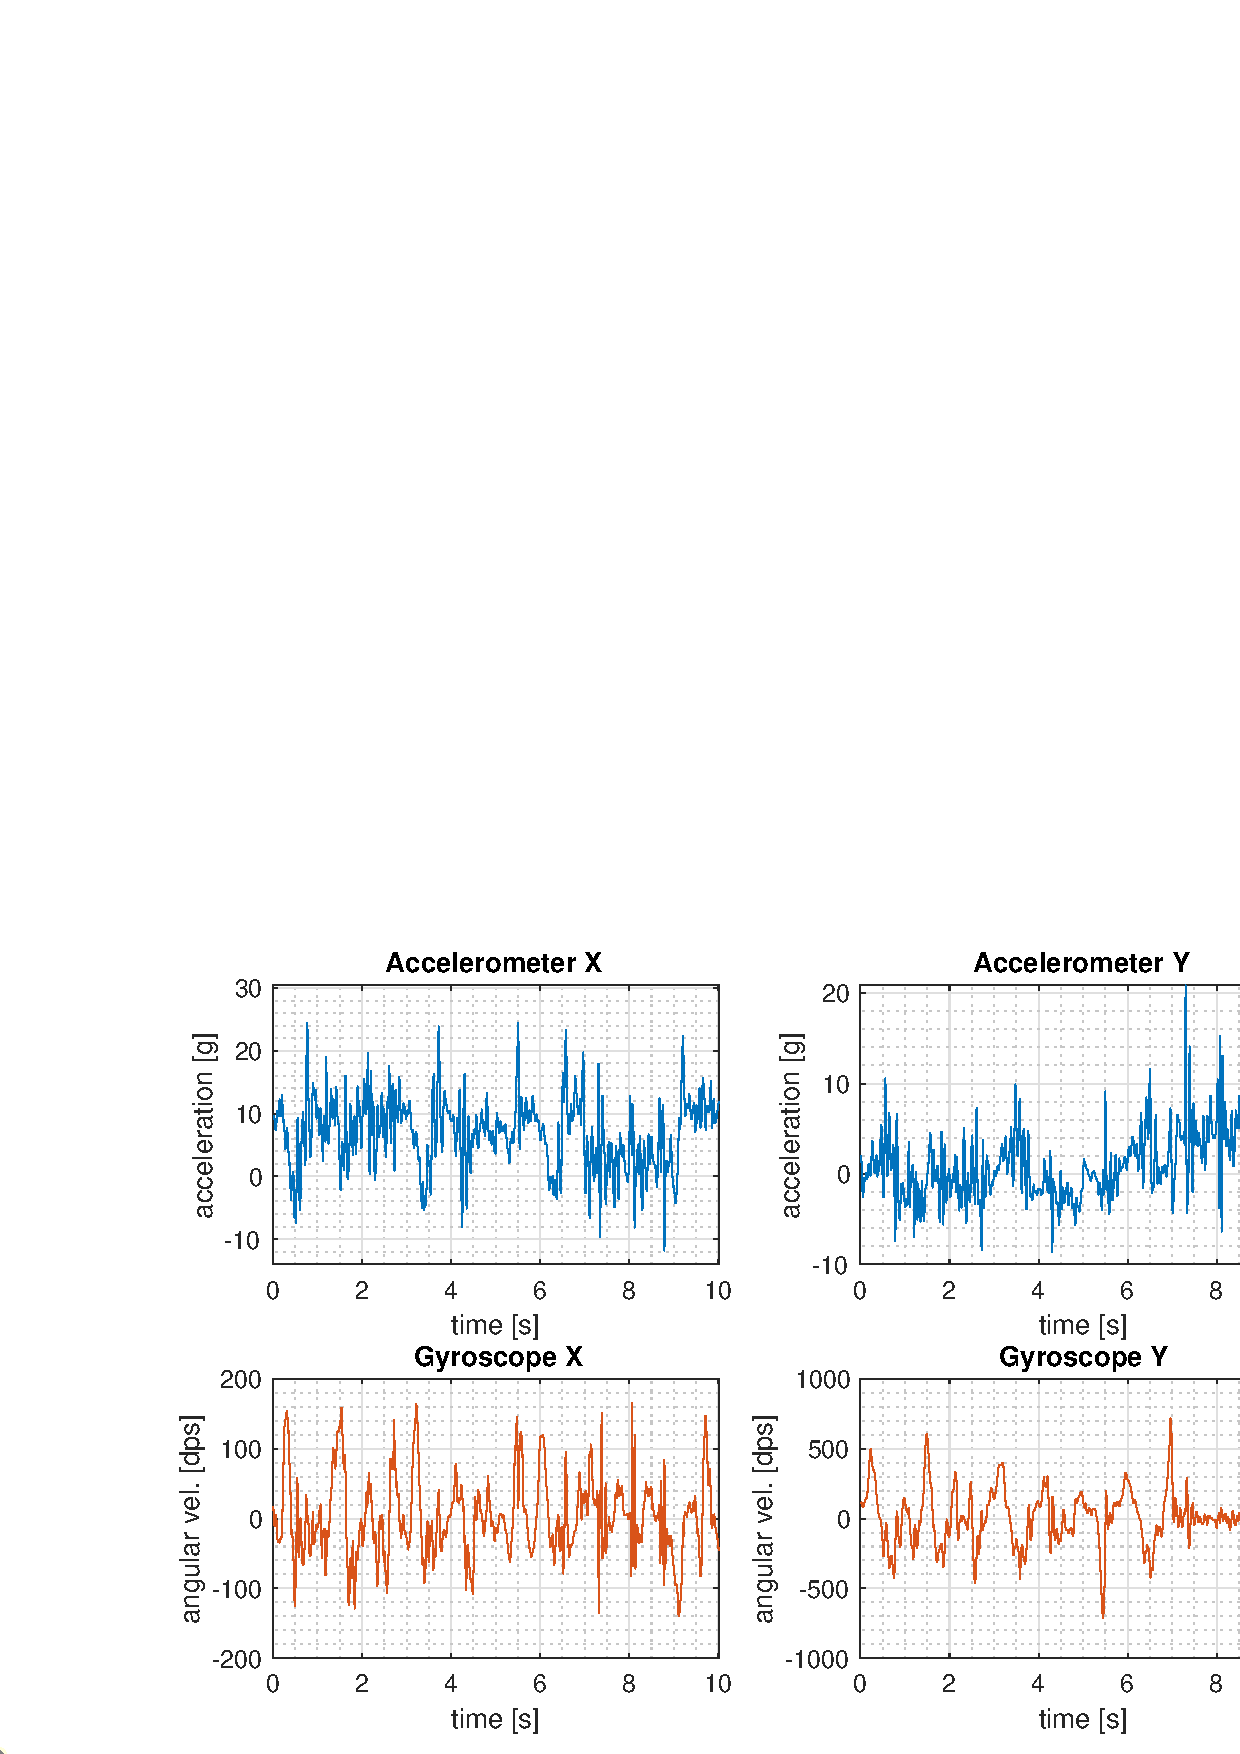
\includegraphics[width=\textwidth]{figure/acc_gyr_plot.pdf}
    \caption{Tracce di accelerometro e giroscopio prodotte durante un'attività di sanificazione delle mani.}
    \label{fig:acc-gyro-plot}
\end{figure}

\`E importante notare che i soggetti non sono istruiti sulla corretta maniera in cui lavare o sanificare le mani e sono stati lasciati completamente liberi di usare il loro metodo abituale in modo da raccogliere dati il più possibile non strutturati. La Tabella \ref{tab:activity-duration} mostra la durata media e la deviazione standard degli eventi di lavaggio e sanificazione per ognuno dei quattro soggetti assieme ad una media e deviazione standard cumulativa. Come si può notare la durata media dipende significativamente dal soggetto.

\begin{table}
    \centering
    \begin{tabular}{c c c}
        \hline
        soggetto & lavaggi & sanificazioni  \\
        \hline
        0 & $66.68s \pm 18.69s$ & $23.66s \pm 6.26s$  \\
        1 & $31.92s \pm 8.97s$  & $26.09s \pm 3.67s$  \\
        2 & $39.47s \pm 8.52s$  & $19.18s \pm 4.29s$  \\
        3 & $30.54s \pm 6.17s$  & $25.44s \pm 8.59s$ \\
        \hline
        media & $50.92 \pm 22.29s$  & $23.59 \pm 7.33s$ \\
        \hline
    \end{tabular}
    \caption{Durata delle attività registrate dal dataset ad hoc in secondi.}
    \label{tab:activity-duration}
\end{table}

Il secondo dataset preso in considerazione è il Daily Living Activities (DLA) che è uno dei pochi dataset disponibili contenente dati di lavaggi di mani campionati attraverso sensori inerziali. Questo dataset è stato creato registrando diverse parti del corpo ed utilizzando differenti sensori indossabili; in particolare dal polso, dai fianchi e dalle caviglie di otto volontari in salute con età compresa fra i 23 e i 37 anni. Il dataset è composto da 17 differenti attività di uso comune, ma, poiché il nostro scopo è valutare i lavaggi delle mani abbiamo filtrato solo i dati raccolti dal polso e rimosso tutte quelle azioni che non hanno a che vedere con le mani. In questo dataset non sono presenti dati raccolti durante la sanificazione, inoltre i sensori utilizzati per la raccolta non sono equipaggiati con un giroscopio il chè può sembrare svantaggioso, ma ci consente di soppesare l'utilità dei segnali del giroscopio e di valutare l'abilità dei modelli proposti nel generalizzare.

\section{Le finestre di campionamento}
\label{sec:le-finestre-di-campionamento}

Le tracce raccolte dal dataset costruito ad hoc sono composte da sei segnali distinti, tre per l'accelerometro e tre per il giroscopio, mentre quelle del dataset DLA hanno solo tre tracce per l'accelerometro; in entrambi i casi le tracce sono state suddivise in finestre ognuna delle quali è considerata come un campione da usare per l'addestramento dei modelli. Ogni campione è stato etichettato durante la fase di raccolta dei dati marchiandolo con un'etichetta che rappresenta il soggetto ed una che rappresenta la categoria di azione compiuta fra queste: lavaggio, sanificazione, altro.

Decidere la dimensione della finestra è un'operazione non semplice poiché influisce sulle performance dei modelli in molti modi diversi; infatti, dev'essere larga abbastanza per includere informazioni significative sulla singola attività, ma non dev'essere troppo grande da includere multipli eventi successivi. Nell'ambito del riconoscimento delle attività umane sono state utilizzate finestre di diversa lunghezza, da 1 secondo fino a 30 secondi\cite{cheng2010active}\cite{hassan2018robust}; in alcuni casi si è arrivati addirittura a finestre piccolissime (solo 0.06 secondi) con un overlap del 70\% fra di loro in modo da riconoscere ogni passaggio della procedura strutturata.

In questa ricerca non dovendoci preoccupare del riconoscimento di dati strutturati abbiamo valutato finestre di dimensione maggiore: dai 2 secondi fino ai 20 secondi e senza overlap fra le finestre. Inoltre, a causa del protocollo di raccolta dei dati proposto, che punta a campionare continuamente i sensori, il numero di altri eventi rispetto ai lavaggio/sanificazioni è di gran lunga maggiore, per questo motivo i campioni etichettati come altro sono stati randomicamente selezionati e ridotti di numero per ri-bilanciare il dataset.

\section{I Classificatori}
\label{sec:classificatori}

Per addestrare e testare l'accuratezza dei modelli di machine learning tradizionali i segnali in input devono essere processati in modo da estrarre una serie di feature significative; in questo lavoro abbiamo delineato tre tipologie di feature. La prima categoria è composta dalle feature Base, ovvero dei descrittori statistici classici come:

\begin{enumerate}
    \item media
    \item deviazione standard
    \item massimo e minimo
    \item mediana
\end{enumerate}

i quali descrivono la tendenza dei campioni, la seconda categoria è quella delle feature Hjorth formata da:

\begin{enumerate}
    \item attività
    \item mobilità
    \item complessità
\end{enumerate}

che catturano le caratteristiche principali del segnale nel dominio della frequenza rappresentando la potenza del segnale e la sua frequenza media, mentre la terza categoria è quella delle feature Shape formata da:

\begin{enumerate}
    \item curtosi 
    \item skewness
\end{enumerate}

con l'obbiettivo di descrivere la forma dei dati, ovvero quanto i dati in esame si discostano da una distribuzione normale.

Nel caso degli approcci di deep learning non è necessario eseguire l'estrazione delle feature utilizzando direttamente i campioni dei segnali divisi in finestre come input della classificazione. Per quanto riguarda la CNN, che comunemente è applicata all'analisi delle immagini, è necessario un passaggio di preprocessing che converte i dati delle serie temporali in un formato visuale. Questa possibilità ha recentemente attratto grande attenzione in letteratura portando alla nascita di diverse strategie di conversione; in questo studio ci concentriamo su un metodo che codifica i dati delle serie temporali in immagini chiamato Gramian Angular Summation/Difference Field(GASF, GADF)\cite{wang2015imaging}. Questo metodo rappresenta le serie temporali in un sistema di coordinate polari, invece delle tipiche coordinate Cartesiane, con il vantaggio di mantenere intatte le relazioni spaziali e temporali. 

Poiché questo approccio porta ad avere due immagini per asse, una per il Gramian Angular Summation(GASF) e l'altra per il Gramian Angular Difference(GADF), nel caso del dataset ad hoc otteniamo un set di 12 immagini, mentre nel caso del dataset DLA solo 6; di conseguenza il modello CNN(Figura \ref{fig:models:cnn}) prende come input un'immagine quadrata a 12 o 6 canali costruita a partire dai dati della finestra e la cui altezza e larghezza dipendono dalla dimensione della finestra (WS). L'immagine è quindi convoluta attraverso quattro livelli convoluzionali di dimensione decrescente intermezzati da livelli di normalizzazione, ReLu e max pooling che hanno l'effetto di stabilizzare il processo di apprendimento diminuendo il numero di epoche richieste. L'output è poi passato attraverso tre livelli densamente connessi ed un Softmax che hanno lo scopo di assegnare ad ogni classe una probabilità proporzionale al segnale di output.

\begin{figure}[!htb]
    \centering
    \begin{subfigure}{\textwidth}
        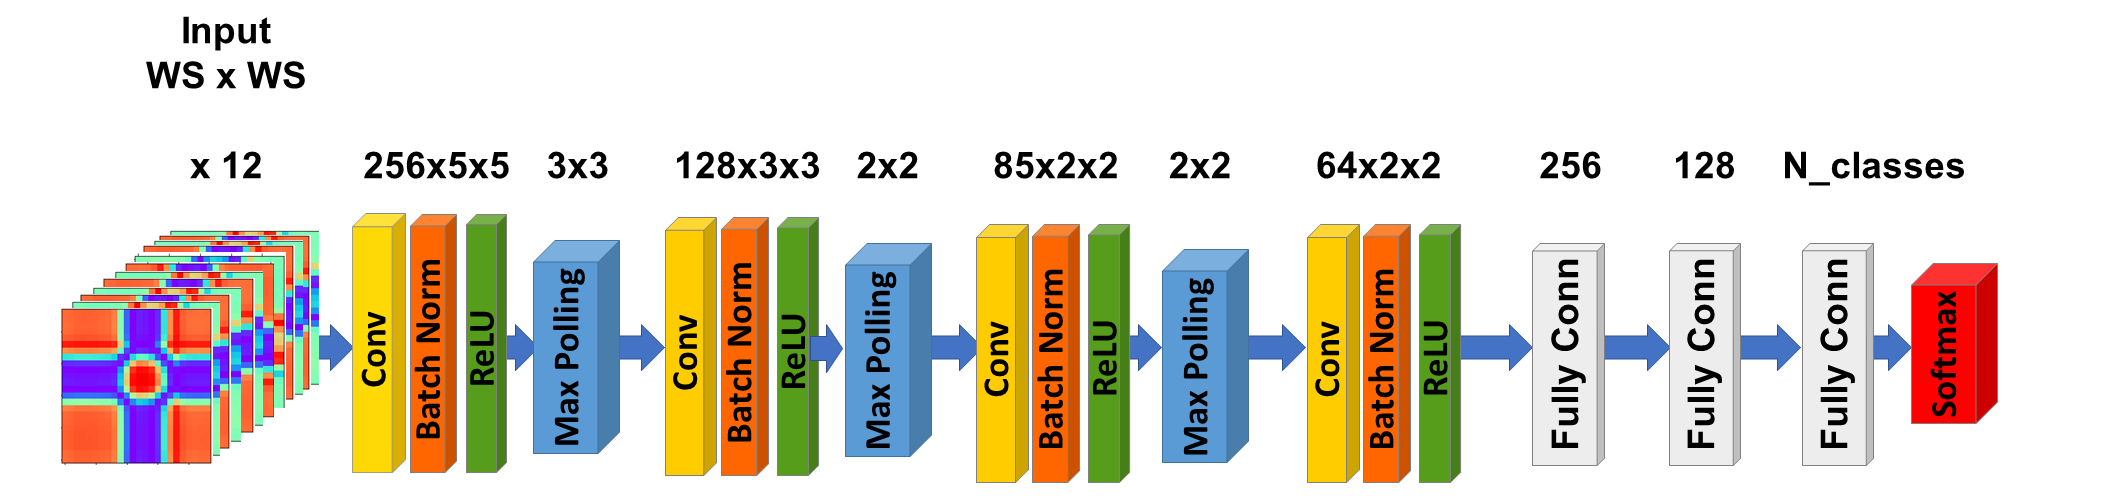
\includegraphics[width=\textwidth]{figure/cnn_model.png}
        \caption{architettura del modello CNN}
        \label{fig:models:cnn}
    \end{subfigure}
    \begin{subfigure}{\textwidth}
        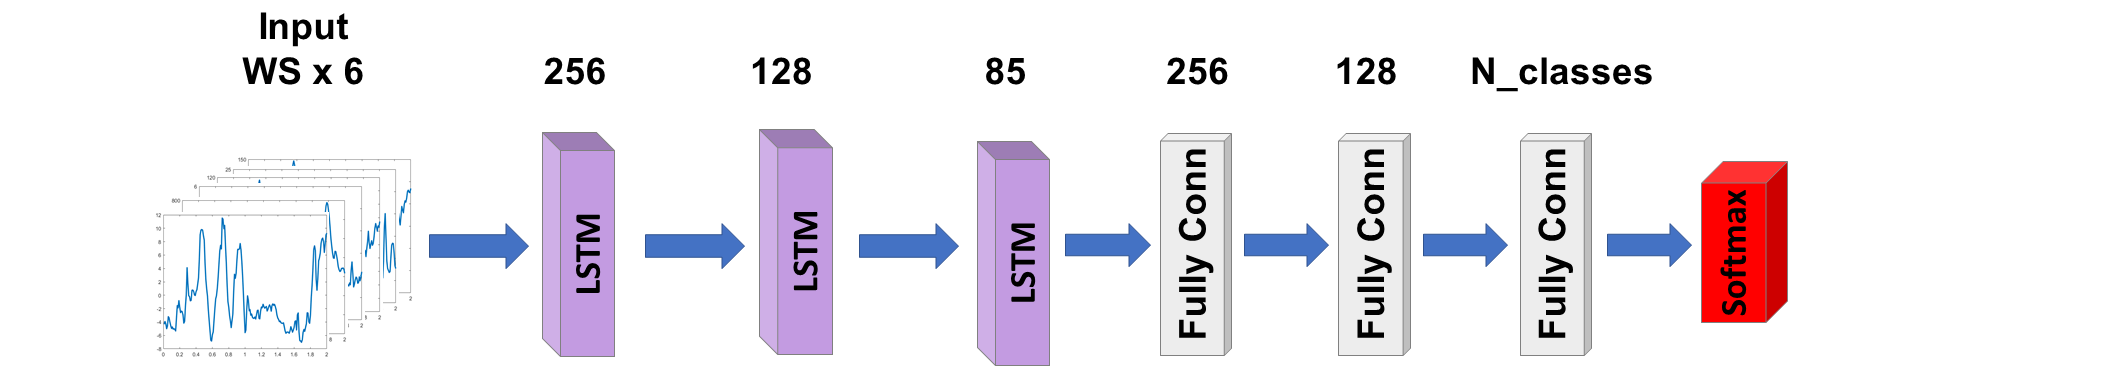
\includegraphics[width=\textwidth]{figure/lstm_model.png}
        \caption{architettura del modello LSTM}
        \label{fig:models:lstm}
    \end{subfigure}
    \caption{Architettura dei modelli di deep learning proposti: CNN(\subref{fig:models:cnn}) e LSTM(\subref{fig:models:lstm}).}
    \label{fig:models}
\end{figure}

D'altro canto la rete LSTM(Figura \ref{fig:models:lstm}) riceve in input le sei sequenze(tre nel caso del DLA) originali della serie temporale la cui lunghezza dipende dalla dimensione della finestra(WS); l'input è poi processato da tre livelli LSTM con numero di unità decrescente ed il loro output è passato in tre livelli densamente connessi che, come nel caso della CNN, si comportano come un Perceptron ricavando una singola classe.

\section{Metriche dei classificatori}
\label{sec:metriche-dei-classificatori}

Per valutare la qualità dei modelli proposti effettuiamo un test di k-fold cross-validation con $k=5$ dal quale ricaviamo una matrice di confusione e gli indicatori $TP_i$, $TN_i$, $FP_i$, $FN_i$, con $i \in [1\cdots N]$, dove $i$ è un indice che identifica la classe specifica trattandosi di classificatori multi-classe; in particolare, $TP_i$ è il numero di veri positivi per la classe $i$, $TN_i$ è il numero di veri negativi, $FP_i$ è il numero di falsi positivi ed $FN_i$ è il numero di falsi negativi. Da questi identificatori abbiamo in seguito ricavato le vere e proprie metriche di qualità: 

\begin{equation}
    Precision = \dfrac{1}{N} \sum_{i=1}^{N} \dfrac{TP_i}{TP_i + FP_i}
    \label{eq:precision}
\end{equation}

\begin{equation}
    Recall = \dfrac{1}{N} \sum_{i=1}^{N} \dfrac{TP_i}{TP_i + FN_i}
    \label{eq:recall}
\end{equation}

\begin{equation}
    Accuracy = \dfrac{1}{N} \sum_{i=1}^{N} \dfrac{TP_i + TN_i}{TP_i + TN_i + FP_i + FN_i}    
    \label{eq:accuracy}
\end{equation}

\begin{equation}
    F1_{score} = 2 \cdot \dfrac{Precision \cdot Recall}{Precision + Recall}
    \label{eq:f1}
\end{equation}

\section{Porting dei modelli sullo smartwatch}
\label{sec:porting-dei-modelli-sullo-smartwatch}

In questa sezione vediamo nel dettaglio il porting dei modelli di machine learning sul dispositivo indossabile HEXIWEAR; come detto nella Sezione \ref{sec:hexiwear} questo smartwatch ha al suo interno 1024KB di memoria Flash e 256KB di memoria RAM, il che, visto il trend dei moderni dispositivi mobile, non è una grande quantità di memoria, infatti sul mercato già in questo momento sono disponibili smartwatch che hanno a disposizione addirittura più di 1GB di memoria RAM, ma il loro costo è molto superiore, fanno uso di un ambiente di sviluppo proprietario più restrittivo ed hanno un consumo di energia tale che la batteria generalmente dura meno di una giornata.

Per via di queste limitazioni fisiche abbiamo dovuto modificare i modelli descritti in precedenza restringendone la struttura e riducendo il numero di parametri da addestrare, ma, nonostante svariati tentativi, siamo stati comunque costretti a scartare i modelli di CNN e ERS-KNN lasciando solo SVM ed LSTM, ma, appartenendo il primo alla categoria di machine learning classica ed il secondo a quella di deep learning, siamo comunque in grado di valutare entrambe le categorie. Nel caso del CNN il fattore limitante è la memoria richiesta sia per contenere tutti i pesi dei parametri della rete che per salvare ed elaborare le 12 immagini GASF/GADF; nel caso dell'ERS-KNN invece, non siamo stati in grado di trovare nessuna libreria che eseguisse l'inferenza sfruttando la tecnica di Ensemble Random Subspace direttamente sui dispositivi embedded e consumando poche risorse.

Per eseguire i modelli sullo smartwatch sono state utilizzate due librerie: TensorFlow 2.0 Lite Micro e libSVM.
TensorFlow è una libreria open-source sviluppata da Google nel 2015 per facilitare le ricerche sul machine learning e le intelligenze artificiali; supporta vari tipi di tecnologie, ma si concentra particolarmente sull'addestramento e l'inferenza di reti neurali profonde(deep neural networks)\cite{abadi2016tensorflow}. In particolare, per l'inferenza sull'HEXIWEAR abbiamo utilizzato TensorFlow 2.0 Lite Micro, una versione di TensorFlow 2.0 pensata appositamente per l'ambito mobile ed i micro-controllori. 
LibSVM\cite{chang2011libsvm} è una libreria di machine learning open-source sviluppata dalla National Taiwan University e scritta in C++ con l'obbiettivo di semplificare l'utilizzo dei modelli SVM da parte di sviluppatori non specializzati. LibSVM supporta sia la classificazione(C-SVC, nu-SVC) che la regressione(epsilon-SVR, nu-SVR) offrendo varie funzionalità tra cui: efficiente classificazione multi-classe, cross-validation con k-fold, strumenti per la stima delle probabilità, supporto per diversi tipi di kernel ed estensioni per interagire con i più comuni linguaggi di programmazione.

In Figura \ref{fig:lstm-models-port} possiamo vedere la struttura dei modelli LSTM dopo la riduzione in cui è presente un solo livello LSTM seguito da due livelli densamente connessi ed un Softmax per convertire i pesi interni in un'etichetta di classificazione. Su questa rete abbiamo condotto un esperimento tenendo fissa la lunghezza della finestra di processing e variando il numero di parametri interni della rete.

Per quanto riguarda l'SVM nella fase di addestramento abbiamo pre-calcolato le feature ed abbiamo addestrato i modelli su un loro sottoinsieme equamente distribuito di 2000 sample, in questo modo abbiamo ridotto notevolmente il peso complessivo dei modelli potendoli caricare in memoria; in questo caso abbiamo condotto due tipologie di esperimenti: uno variando la lunghezza della finestra di processing e l'altro variando il numero di feature calcolate.

\begin{figure}[!htb]
    \centering
    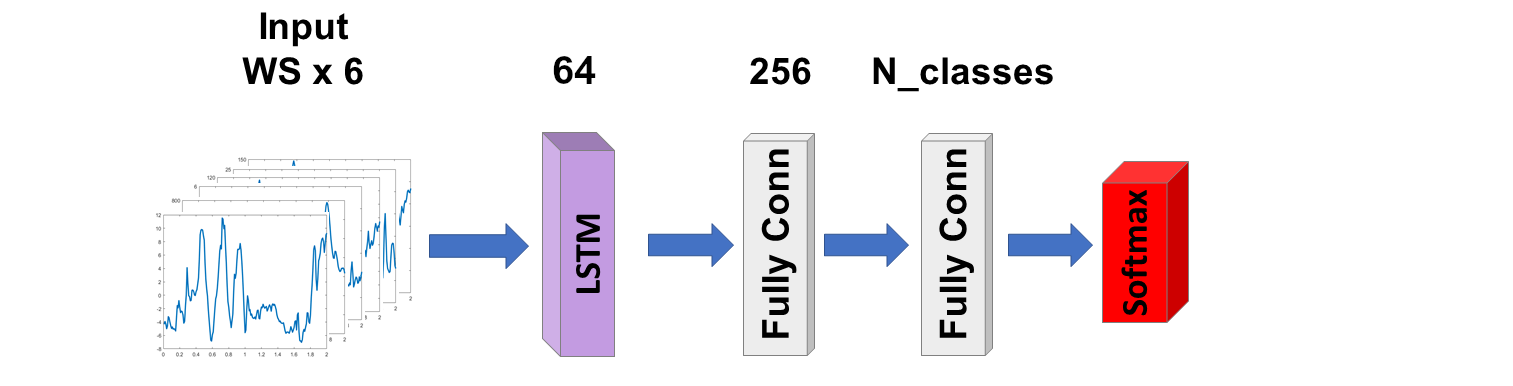
\includegraphics[width=\textwidth]{figure/lstm_model_64.png}
    \caption{Modello LSTM ridotto per il porting sullo smartwatch HEXIWEAR.}
    \label{fig:lstm-models-port}
\end{figure}